\chapter{Methodology}
\label{chapter:methodology}
To perform \unity{} performance bug analysis, we collected real-world bugs from GitHub projects. With the collected performance bug fix data, we performed i) Root cause analysis, ii) Code change-based AST diff analysis, and iii) Commit Analysis. Figure~\ref{figure:overview} shows overview of our overall methodology. In the subsequent sections, we discussed each of the components of our methodology.


\begin{figure*}[t]
	%%\vspace{-0.2cm}
	\centering
	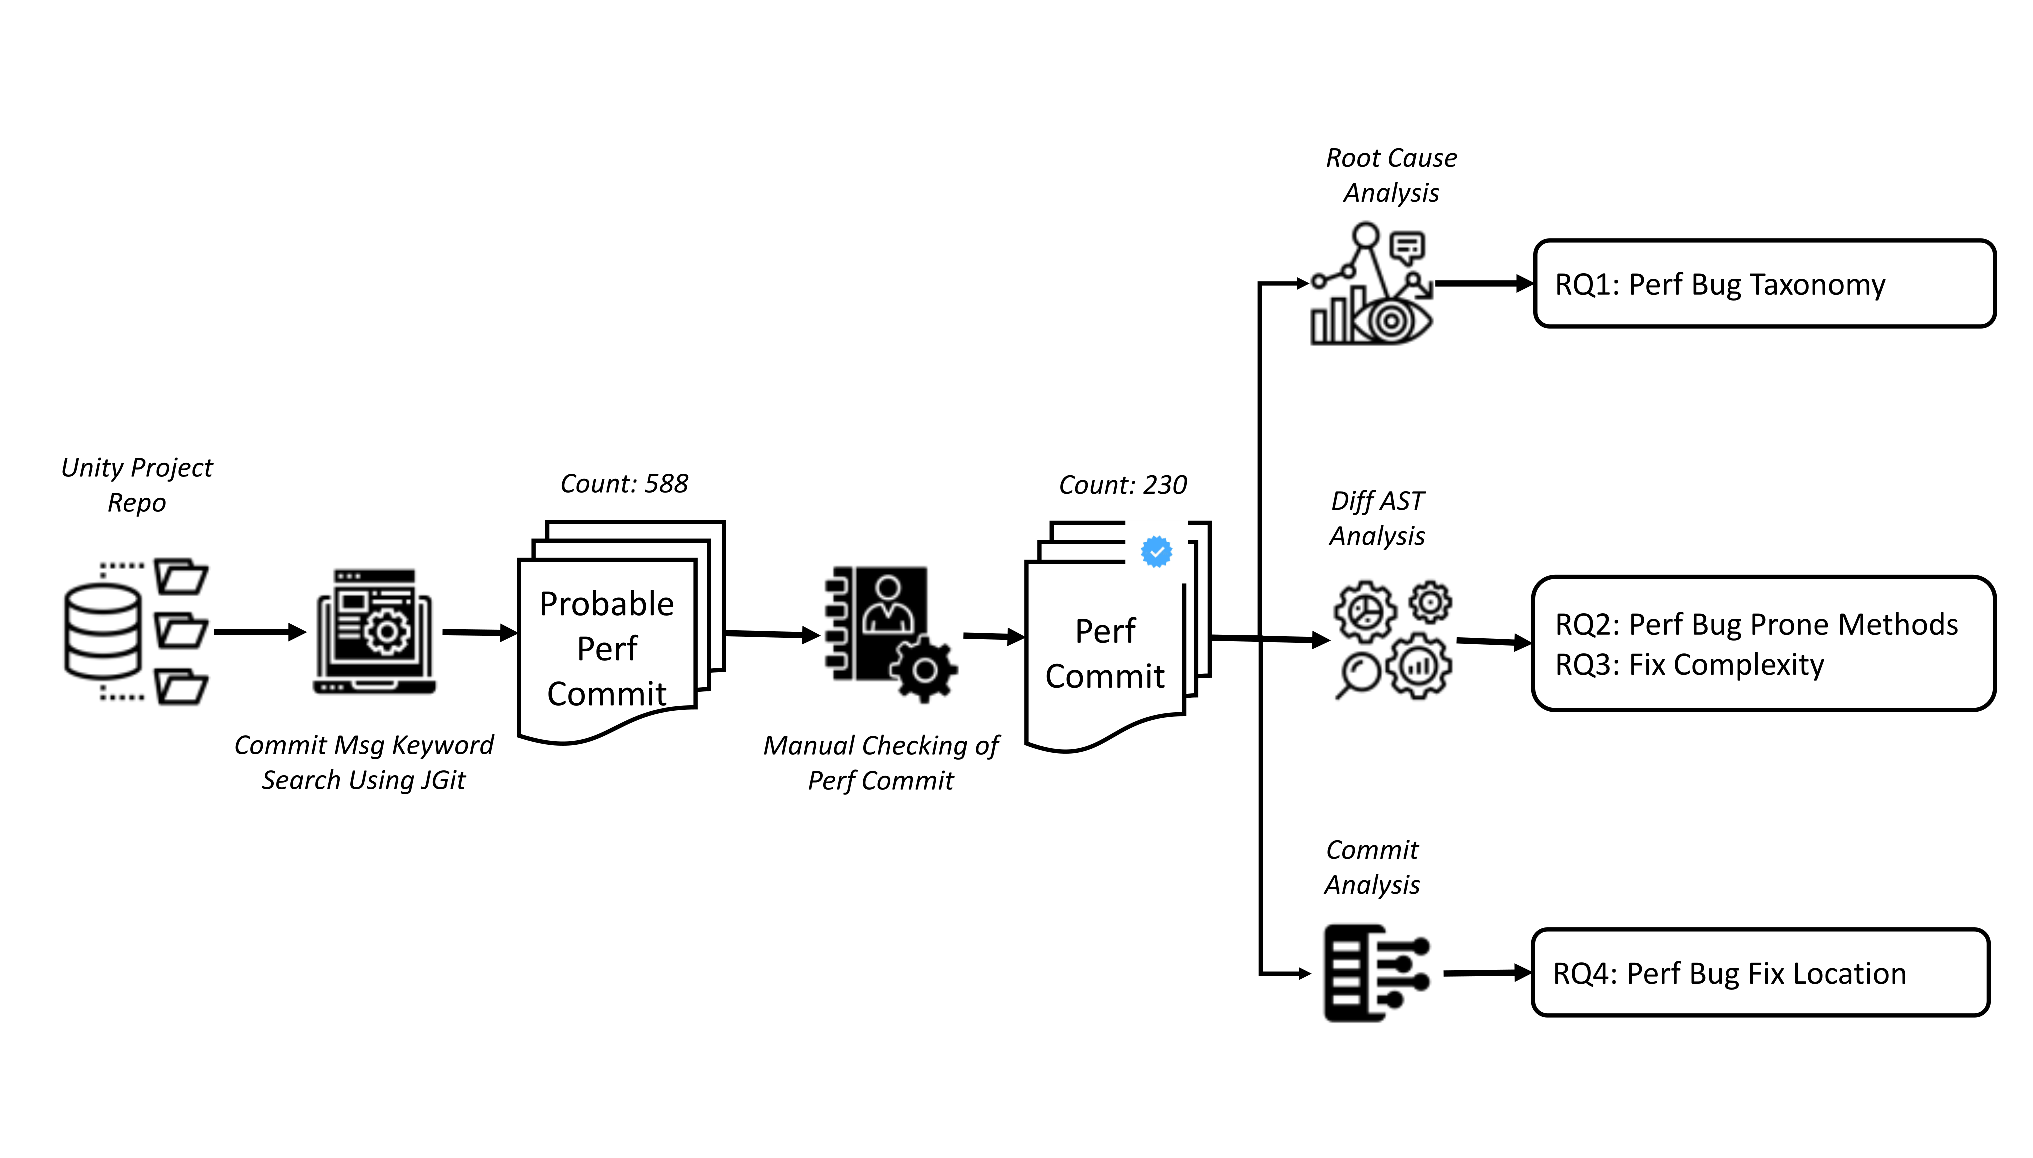
\includegraphics[width=0.9\textwidth]{figure/overview.eps}
	%\vspace{-0.3cm}
	\caption{Overview of Unity Performance Bug Analysis}
	%	\vspace{-0.3cm}	
	\label{figure:overview}
\end{figure*}

\section{Unity Performance Bug Data Collection}
\label{sec:datacollection}
For Data Collection, we collected 100 Github projects with more than 100 commits. We used the commit threshold to ensure that the projects are well maintained and have sufficient fixed data. With these 100 projects, we programmatically searched for performance fix related keywords in commit message using Java Git library JGit~\cite{JGit}. As part of keyword search, we used \textbf{performance}, \textbf{speed up}, \textbf{accelerate}, \textbf{fast}, \textbf{slow}, \textbf{latency}, \textbf{contention}, \textbf{optimize}, and \textbf{efficient} keywords as search token. Prior research~\cite{Chen:perf:19} on performance bug also used these keywords to find performance related bug fix. With this search strategy, we identified 588 probable performance-related issues. Later we manually checked the commits for the performance-related fix. We checked the commit messages thoroughly and also the fix for performance fix correctness. With our analysis, we identified 230 actual performance related bug fix. Since for Unity, we did not have any dataset for performance analysis, this dataset can contribute to further research on unity performance-related bugs.


\section{Root Cause Analysis}
\label{sec:rootcause}
With detailed root cause analysis, we identified Unity's performance bug fix taxonomy. That means, we categorized the bugs depending on their types and how they got fixed. We categorized these 230 bugs into 15 categories.






\section{Code change-based AST diff analysis}
\label{sec:diffanalysis}
For change/diff based analysis, we performed AST (Abstract Syntax Tree) level diff analysis. For C\# AST tree generation, we did not find any opensource parser. So, we  used srcML~\cite{srcML} a generic parsing research tool. With srcML, we converted C\# code into XML format code. Then we loaded those XML format code and performed AST level diff with the state of the art diff tool GumTree~\cite{Jean:gumtree:2014}. With this approach, we can extract AST level code changes. Figure~\ref{figure:astdiff} shows the overview of C\# AST level diff analysis.

\begin{figure*}[t]
	%%\vspace{-0.2cm}
	\centering
	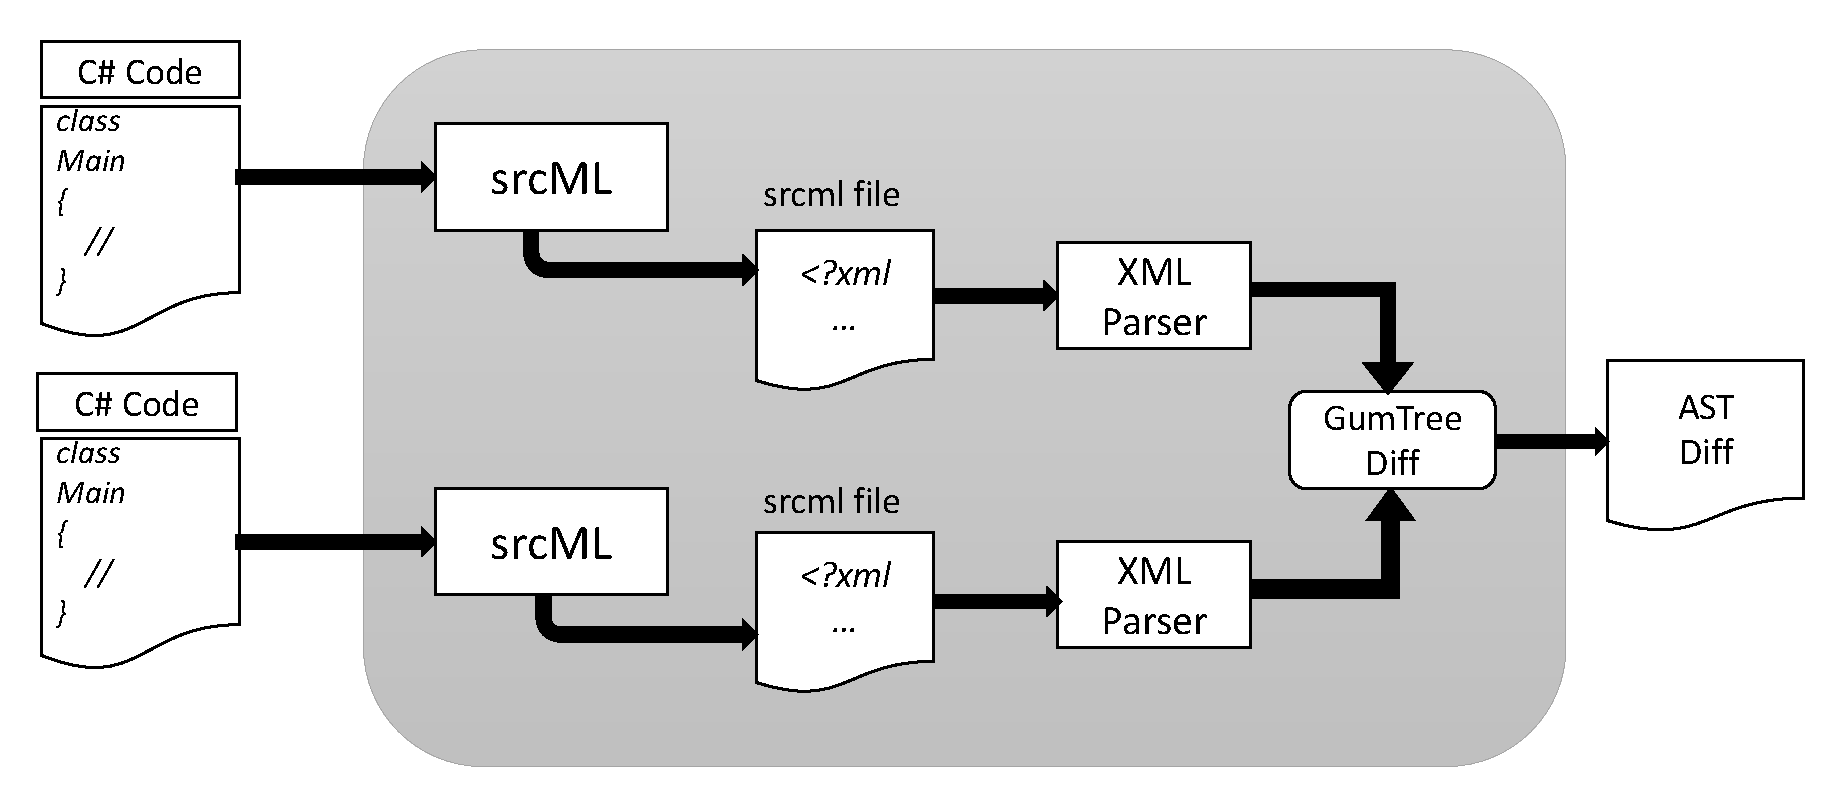
\includegraphics[width=0.9\textwidth]{figure/diff_overview.eps}
	\caption{C\# AST Level Diff Generation}
	\label{figure:astdiff}
\end{figure*}

Here is an example of the AST diff that we generated using our approach. We keep track of class name, method name, action such as insert, delete move etc. Also label and type. For example, here the class name is Answer, no function is used. And there is a single expression, whose type is "using name operator name", and label is "UnityEngine.UI". This "using" in C\# is equivalent to Java "import". Also there is an "insert" action. 


\definecolor{gray}{rgb}{0.4,0.4,0.4}
\definecolor{darkblue}{rgb}{0.0,0.0,0.6}
\definecolor{cyan}{rgb}{0.0,0.6,0.6}

\lstset{
	basicstyle=\ttfamily,
	columns=fullflexible,
	showstringspaces=false,
	commentstyle=\color{gray}\upshape
}

\lstdefinelanguage{XML_android}
{
	morestring=[b]",
	morestring=[s]{>}{<},
	morecomment=[s]{<?}{?>},
	stringstyle=\color{black},
	identifierstyle=\color{darkblue},
	keywordstyle=\color{cyan},
	morekeywords={xmlns,version,type}% list your attributes here
}

\begin{example}
\begin{lstlisting}[language=XML_android, basicstyle=\ttfamily\footnotesize, numbers=left, numbersep=5pt, captionpos=b]
<?xml version="1.0" encoding="UTF-8" standalone="no"?><patch id="3">
	<classname name="Answer">
		<funcname name="">
			<stmt id="1">
				<exp id="0">
					<type>using name operator name </type>
					<label>  UnityEngine . UI </label>
					<action>insert</action>
				</exp>
			</stmt>
		</function>
	</classname>
</patch>
	\end{lstlisting}
	\caption{C\# Code Differencing Output Format}
		%\scriptsize{\textit{(BuildCraft/BuildCraft: 98f7196)}}}
	\label{example:changerep}
	\vspace{-0.2cm}
\end{example}

With AST level code changes, we analyzed which methods are prone to performance bug and the complexity of performance bug fix. We categorized performance bug fix methods as Unity Callback, Custom Callback, and User Defined Method during the analysis of performance bug-prone methods. Unity Callbacks are unity provided callbacks such as Update. Update method is called in every frame if the MonoBehaviour is enabled. MonoBehaviour is the base class from which every Unity script derives. Similarly, Start is another Unity callback. Custom callbacks are event listeners that developers can add from code. User-Defined Methods are other utility or supporting methods that are used in unity scripts. Apart from that, we also performed analysis for most frequently changed methods. During the most common method change analysis, we performed analyses based on only method body changed based analysis and also method body considering call graph-based analysis.



\section{Commit Analysis}
\label{sec:commitanalysis}
In typical bug fix, we do have a normal illusion that performance bugs are mostly fixed in source code. To analyze the factor, we analyzed the performance fix location. So for the 230 performance bugs, we analyzed git commit. We captured the Delta or change in between bug fix commit and its parent commit. From Delta, we identified which files are changed. Based on file type change, we categorized fix location. We did this analysis programmatically with the help of Git Java library JGit. Figure~\ref{figure:commitanalysis} shows the overview of commit analysis.

\begin{figure*}[t]
	%%\vspace{-0.2cm}
	\centering
	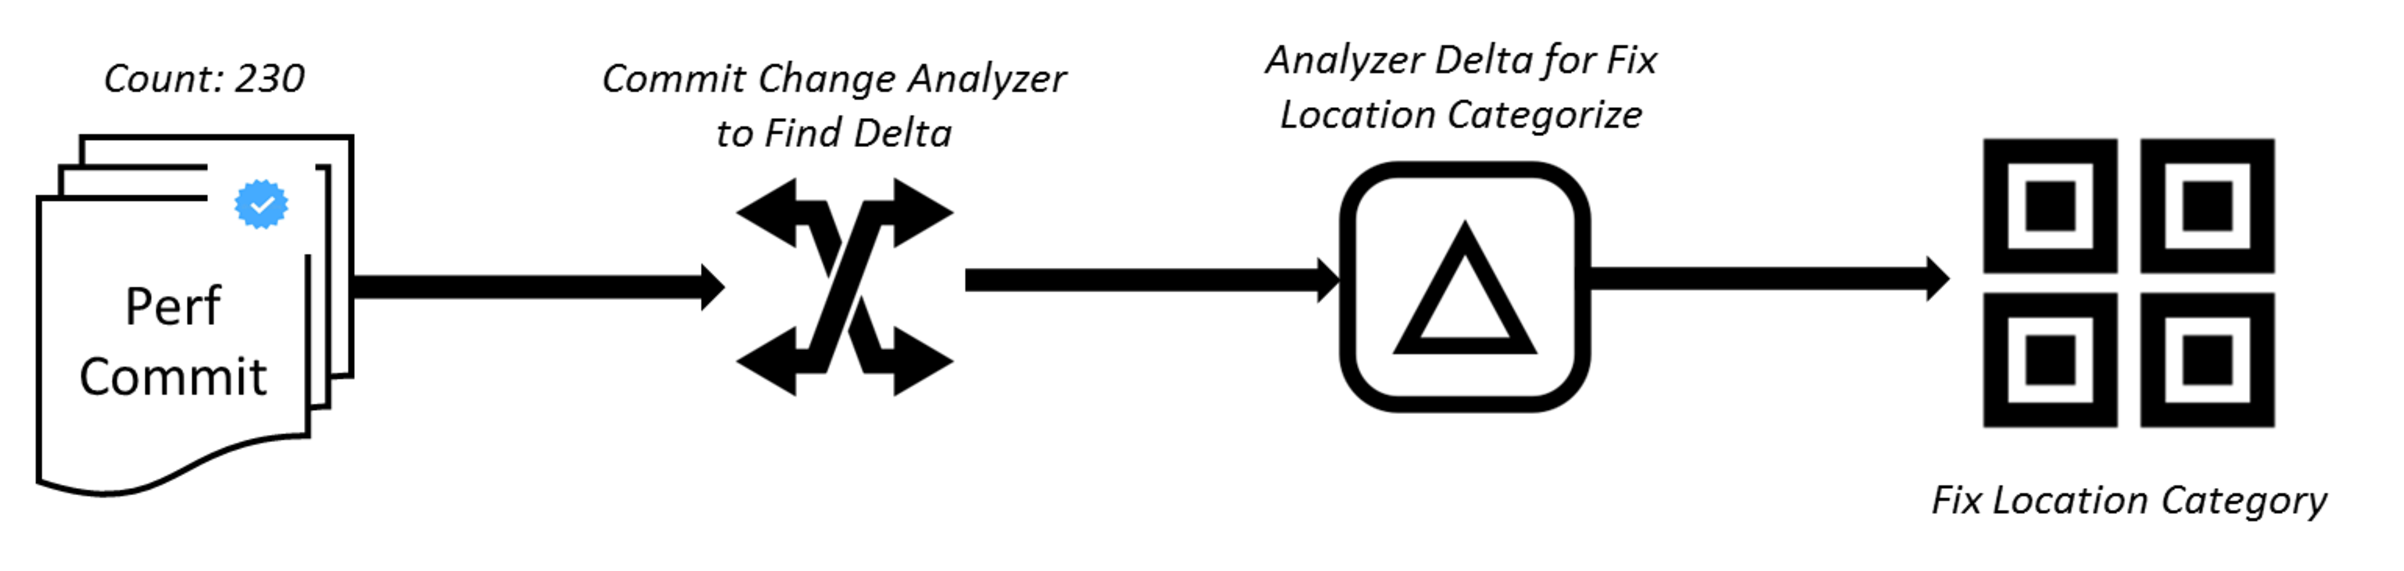
\includegraphics[width=0.9\textwidth]{figure/commitanalysis.eps}
	%\vspace{-0.3cm}
	\caption{Overview of Commit Analysis}
	%	\vspace{-0.3cm}	
	\label{figure:commitanalysis}
\end{figure*}
